\documentclass[tikz]{standalone}
%\documentclass[]{article}
%\usepackage[paperwidth=25in, paperheight=25in]{geometry}
\usepackage{pgf}
\usepackage{tikz}
\usetikzlibrary{automata}
\usetikzlibrary{positioning, fit, shapes, calc}
\usetikzlibrary{decorations.pathreplacing}
\usetikzlibrary{shapes.symbols}
\usepackage{verbatim}
\usepackage{ifthen}
\usepackage{amsmath}


\begin{comment}
:Title: Neural network
:Tags: Foreach

The ``\foreach`` command is very useful for quickly creating structured graphics
like this neural network diagram.

\end{comment}

\begin{document}
	\pagestyle{empty}
%%--------------Initialization section ----------------	
%	% Total number of layers including the input layer and the output layer.
%	\def\layerNumber{4} % Start counting at 0
%	% Number of input features.
%	\def\featureNumber{2} %Start counting at 0 where 0 corresponds to the first bias term of the network.
%	% Number of neurons and bias terms in each hidden layer.
%	\def\neuronsAndBiasPerLayer{2} % Start counting at 0.
%%------------------------------------------------------ 
%	
%	% Distance between layers in cm.
	\def\ticksep{3cm}
%	% Distance between neurons of the same layer.
%	\def\neuronVerticalSeparation{4cm}
%	% Auxiliary indices needed for the plotting functions.
%	\pgfmathtruncatemacro{\lastHiddenLayerNo}{\layerNumber-1}
%	\pgfmathtruncatemacro{\previousThanLast}{\layerNumber-2}
%	%only neurons and starts counting at 1.
%	\pgfmathtruncatemacro{\neuronsPerLayer}{\neuronsAndBiasPerLayer} % Start counting at 1
	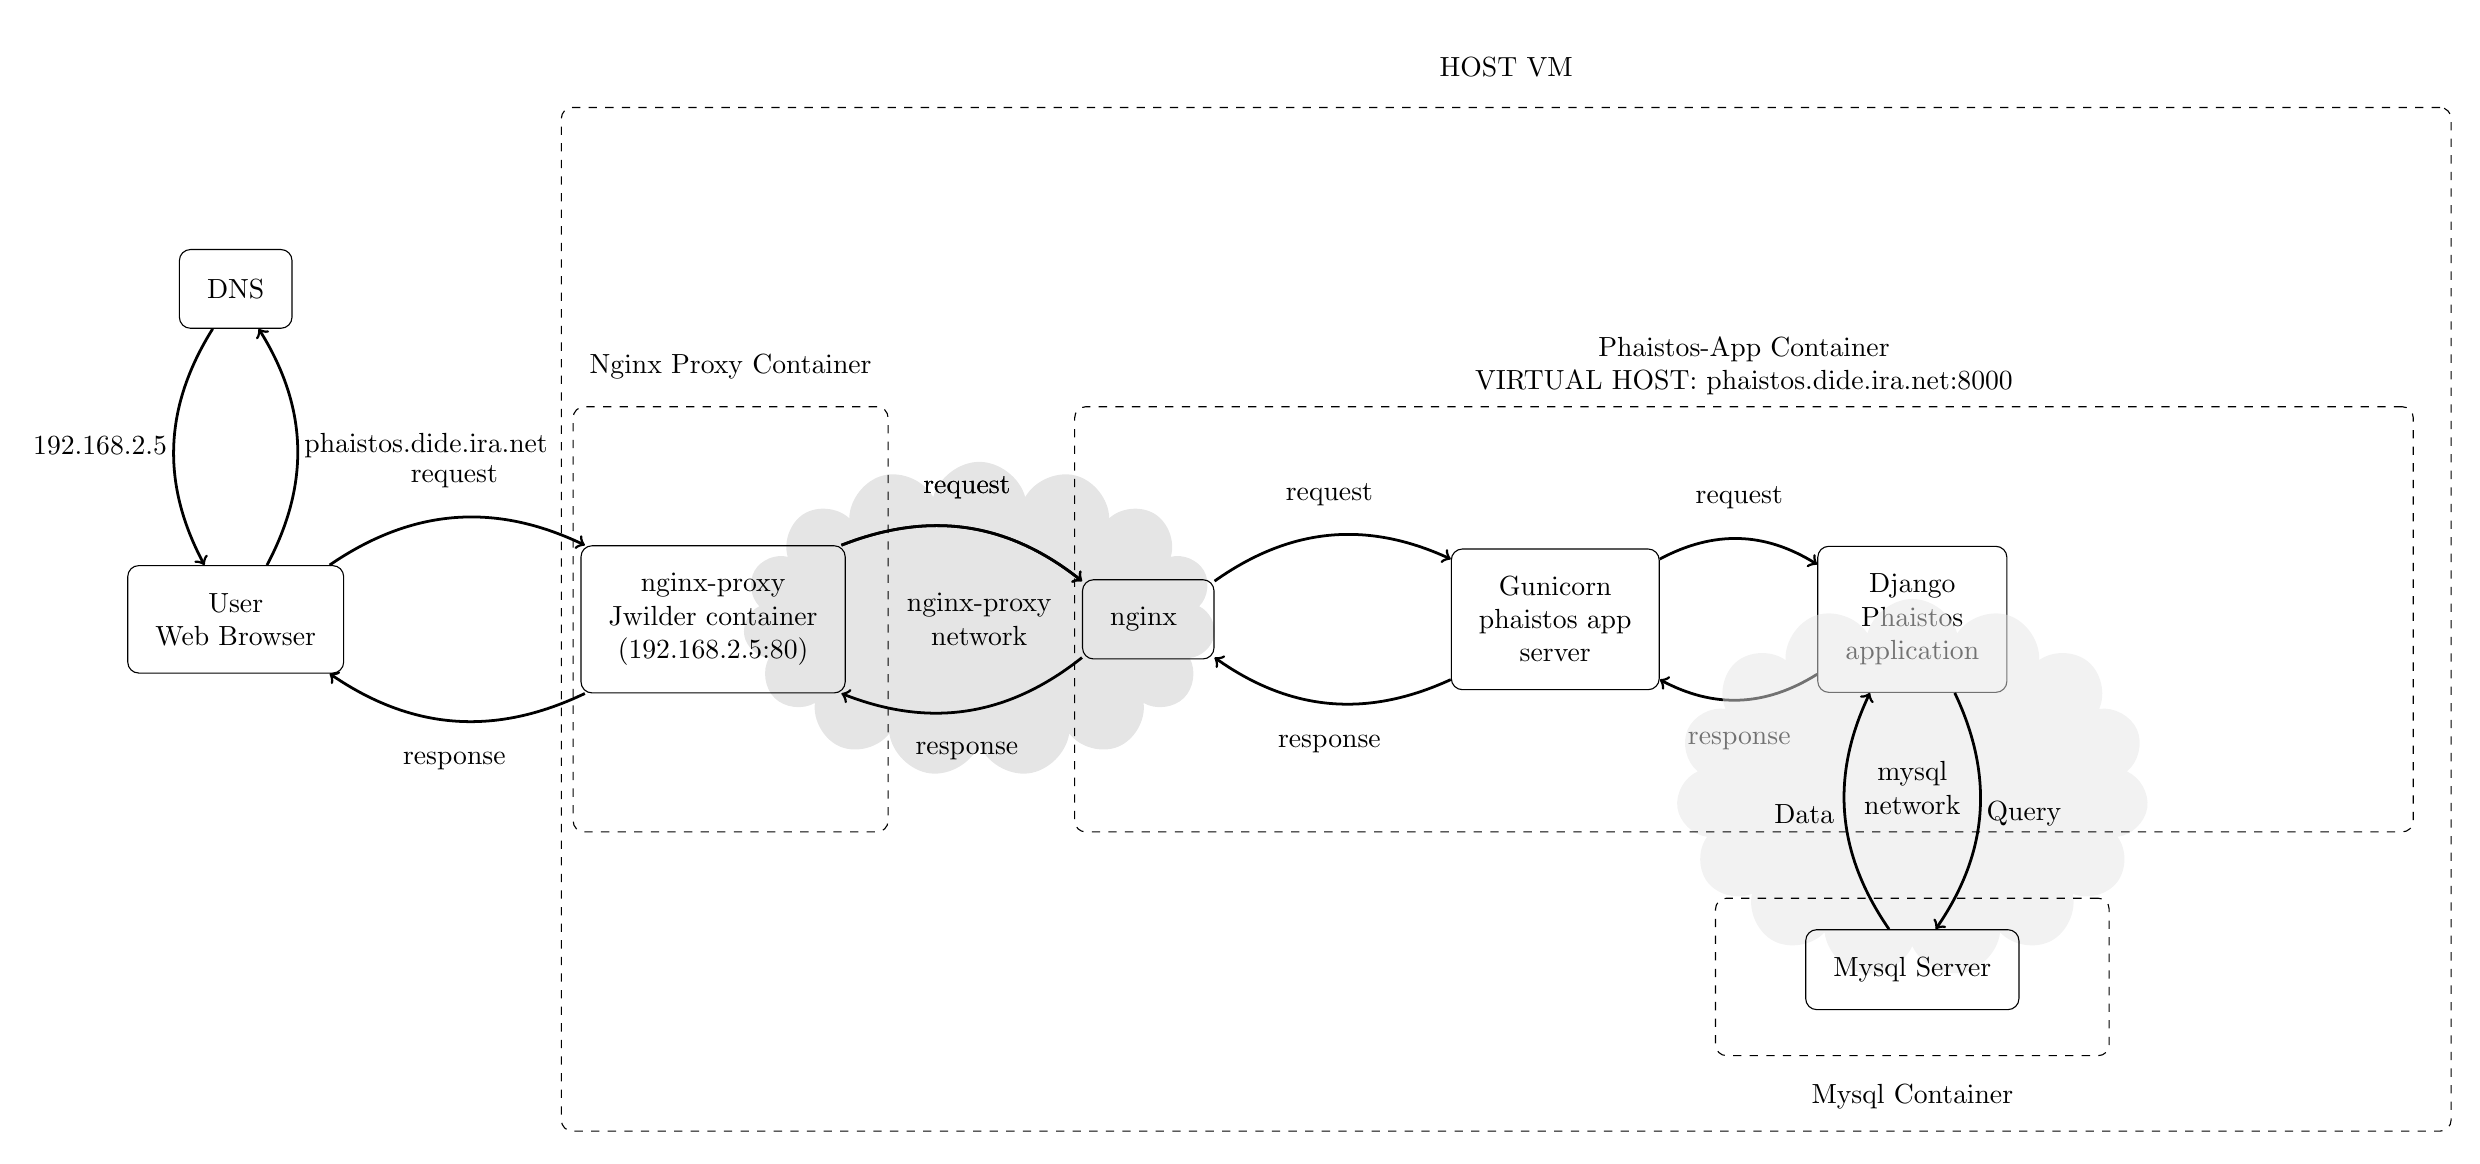
\begin{tikzpicture}[node distance = 3cm, align=center, every node/.style={minimum height=1cm, minimum width = 1cm, inner sep=2pt}]

	\node[draw, rectangle, rounded corners, inner sep=10pt] (DNS) {DNS};

	\node[draw, rectangle, rounded corners, inner sep=10pt, node distance=3cm] (browser)[below=of DNS] {User \\ Web Browser};
	% \node[draw, rectangle, rounded corners, inner sep=10pt] (browser_2)[below =of browser_1] {User Web Browser};
	% \node[draw, rectangle, rounded corners, inner sep=10pt] (browser_3)[below =of browser_2] {User Web Browser};
	\node [cloud, cloud puffs=15, fill=gray!20, behind path, minimum width=6cm, minimum height=4cm] (nginx-proxy-network) [right = 5.1cm of browser] {nginx-proxy\\network};

	\path[draw, line width=1, ->] (browser) edge[bend right] node[right] {phaistos.dide.ira.net} (DNS) ;
	\path[draw, line width=1, ->] (DNS) edge[bend right] node[left] {192.168.2.5} (browser) ;

	\node[draw, rectangle, rounded corners, inner sep=10pt] (nginx-proxy)[right =of browser] {nginx-proxy \\ Jwilder container \\(192.168.2.5:80)};
	% \path[draw, line width=1, ->] (browser) edge[] node[above] {request} (nginx-proxy);
	\path[draw, line width=1, ->] (browser) edge[bend left] node[above] {request} (nginx-proxy);
	\path[draw, line width=1, ->] (nginx-proxy) edge[bend left] node[below] {response} (browser);

	\node[draw, rectangle, rounded corners, inner sep=10pt] (phaistos-nginx)[right =of nginx-proxy] {nginx };
	% \path[draw, line width=1, ->] (nginx-proxy.east) edge[bend left] node[above] {request} (phaistos-nginx.west);
	\path[draw, line width=1, ->] (nginx-proxy) edge[bend left] node[above] {request} (phaistos-nginx);
	\path[draw, line width=1, ->] (phaistos-nginx) edge[bend left] node[below] {response} (nginx-proxy);
	\path[draw, line width=1, ->] (nginx-proxy) edge[bend left] node[above] {request} (phaistos-nginx);	
	% \path[draw, line width=1, ->] (phaistos-nginx) edge[bend left] node[below] {response} (nginx-proxy);

	\node[draw, rectangle, rounded corners, inner sep=10pt] (phaistos-gunicorn)[right =of phaistos-nginx] {Gunicorn \\ phaistos app \\ server};
	\path[draw, line width=1, ->] (phaistos-nginx) edge[bend left] node[above] {request} (phaistos-gunicorn);
	\path[draw, line width=1, ->] (phaistos-gunicorn) edge[bend left] node[below] {response} (phaistos-nginx);

	
	\node[draw, rectangle, rounded corners, inner sep=10pt, align=center, node distance=2cm] (phaistos-django)[right =of phaistos-gunicorn] {Django \\ Phaistos \\ application};
	% \node [cloud, cloud puffs=15, fill=gray!20, behind path, minimum width=6cm, minimum height=4cm] (nginx-proxy-network) [below= -1cm of phaistos-django ] {mysql\\network};

	\path[draw, line width=1, ->] (phaistos-gunicorn) edge[bend left] node[above] {request} (phaistos-django);
	\path[draw, line width=1, ->] (phaistos-django) edge[bend left] node[below] {response} (phaistos-gunicorn);

	\node [cloud, cloud puffs=15, fill=gray!20, behind path, minimum width=6cm, minimum height=4.8cm, text opacity=1, semitransparent] (mysql-network) [below = -1.2cm of phaistos-django] {mysql\\network};

	\node[draw, rectangle, rounded corners, inner sep=10pt, align=center, node distance=3cm] (phaistos-mysql)[below =of phaistos-django] {Mysql Server};
	\path[draw, line width=1, ->] (phaistos-django) edge[bend left] node[right] {Query} (phaistos-mysql);
	\path[draw, line width=1, ->] (phaistos-mysql) edge[bend left] node[left] {Data} (phaistos-django);

	\node[draw, dashed, rectangle, rounded corners, inner sep=10pt, minimum height=13cm, minimum width=24cm] (host-vm)[right = 2.75cm of browser, label=above:HOST VM] {};
	\node[draw, dashed, rectangle, rounded corners, inner sep=10pt, minimum height=5.4cm, minimum width=17cm] (app-container)[right = 2.9cm of nginx-proxy, label=above:Phaistos-App Container \\VIRTUAL HOST: phaistos.dide.ira.net:8000] {};
	\node[draw, dashed, rectangle, rounded corners, inner sep=10pt, minimum height=5.4cm, minimum width=4cm] (nginx-proxy-container)[right = 2.9cm of browser, label=above:Nginx Proxy Container] {};
	\node[draw, dashed, rectangle, rounded corners, inner sep=10pt, minimum height=2cm, minimum width=5cm] (mysql-container)[below = 2.6cm of phaistos-django, label=below:Mysql Container] {};
	% \node[draw, rectangle, rounded corners, inner sep=2pt] (input) at (0,0pt) {Input layer(2)};	
	% \node[draw, rectangle, rounded corners, inner sep=2pt] (hidden_layer_1) at (0,-25pt) {FC(32)};
	% \node[draw, rectangle, rounded corners, inner sep=2pt] (nonlinearity_1) at (0, -50pt) {ReLU};	
	% \node[draw, rectangle, rounded corners, inner sep=2pt] (hidden_layer_2) at (0,-75pt) {FC(64)};
	% \node[draw, rectangle, rounded corners, inner sep=2pt] (nonlinearity_2) at (0, -100pt) {ReLU};	
	% \node[draw, rectangle, rounded corners, inner sep=2pt] (output) at (0,-125pt) {FC(1)};
	% \node[draw, rectangle, rounded corners, inner sep=2pt] (output_nonlinearity) at (0, -150pt) {$\tanh$};
	% \node[draw, rectangle, rounded corners, inner sep=2pt] (tx_power_1) at (0, -175pt) {$P_1 = P_L + \frac{ (\downarrow) + 1}{2} (P_U - P_L)$};
    % % \node[ rectangle, rounded corners, inner sep=2pt] (output_label) at (0, -190pt) {output};
    
	% \path[draw, lightgray, line width=3, ->] (state) edge (input);
	% \path[draw, lightgray, line width=3, ->] (input) edge (hidden_layer_1);
	% \path[draw, lightgray, line width=3, ->] (hidden_layer_1) edge (nonlinearity_1);
	% \path[draw, lightgray, line width=3, ->] (nonlinearity_1) edge (hidden_layer_2);
	% \path[draw, lightgray, line width=3, ->] (hidden_layer_2) edge (nonlinearity_2);
	% \path[draw, lightgray, line width=3, ->] (nonlinearity_2) edge (output);
	% \path[draw, lightgray, line width=3, ->] (output) edge (output_nonlinearity);
	% \path[draw, lightgray, line width=3, ->] (output_nonlinearity) edge (tx_power_1);






%	\node [cloud, draw,cloud puffs=10,cloud puff arc=120, aspect=2, inner ysep=1em] (wan) [right=of monitor] {WAN};
%	\node[draw, rectangle, rounded corners, inner sep=2pt] (edge_device) [right=of wan] {Edge device};
%	\node[draw, rectangle, rounded corners, inner sep=2pt, text width = 163pt, text height=60pt, dotted] (aggregate) at (4.25,0) {};
%	\node[] (network) [above=-20pt of aggregate] {Network};
%	\node[draw, fit=(network) (monitor) (edge_device)] {};	

% 	\node[rectangle, rounded corners, inner sep=2pt] (sensor)  at (4,0) {\includegraphics[width=.1\textwidth]{./sensor.jpg}};
% 	\path[draw,dashed, ->] (input) edge []  node [above=-0.3] {$l_{MS}$} (hidden_layer_1);

% 	\path[draw,line width=3, ->] (hidden_layer_2) edge (nonlinearity_2);


% 	\path[draw,dashed, ->] (input) edge []  node [above=-0.3] {$l_{MS}$} (hidden_layer_1);

% 	\path[draw,dashed, ->] (sensor)  edge [bend left]  node [below=-0.3] {$l_{SM}$} (monitor);
% 	\node[rectangle, rounded corners, inner sep=2pt] (sensor_label) at (4,-30pt) {Sensor};	
%	\path[draw] (monitor) edge [anchor=bend left] node [right] {} (sensor);
%	\path[draw] (monitor) edge [bend right] node [right] {} (sensor);
%	\node[draw, circle] (sensor_1) [above=of sensor_2] {$s_1$};
%	\node[] (sensor_dots) [below=-4pt of sensor_2] {$\vdots$};
	
%	\node[draw, circle] (sensor_3) [below=1pt of sensor_dots] {$s_M$};
	
%	\path[draw] (monitor) -- (wan) -- (edge_device);
%	\foreach \i in {1,...,3}
%		\path[draw, dashed] (sensor_\i) -- (edge_device.east);	
%	\node[inner sep=0pt] (randomProcess) at (-1,0) % {\includegraphics[scale=0.2]{randomProcessExample.pdf}};
%	\node at (-1,1.1cm) {Random Process};
%	\node[draw, circle, minimum size = 1cm ] (transmitter) at (2, 0) {TX} ;
%	\node[draw, rectangle, inner sep=2pt] (channel) at (5, 0) {Channel} ;
%	\node[draw, circle, minimum size = 1cm] (destination) at (8, 0) {D};
%	
%	\node[minimum size=0.1cm] (arrow1_start) at (0.5, 0.35) {};
%%	\node[draw, circle, minimum size=0.1cm] (arrow1_end) at (0.9, -0.25) {};
%	\path[draw, ->] (arrow1_start) arc (65:20:0.7cm);
%	\node[minimum size=0.1cm] (arrow2_start) at (3, 0.35) {};
%	%	\node[draw, circle, minimum size=0.1cm] (arrow1_end) at (0.9, -0.25) {};
%	\path[draw, ->] (arrow2_start) arc (65:20:0.7cm);
%	
%	\draw (1.75cm,2cm) -- (1.75cm,1cm) -- (2.25cm,1cm) -- (2.25cm,2cm);
%	\foreach \i in {1,...,4}
%	\draw (1.75cm, 1cm+\i*5pt) -- (2.25cm,1cm+\i*5pt);
%	\draw[->] (2cm, 1cm) -- (transmitter);
%	\node[] (Battery) at (3.5cm, 1.5cm) {Energy Buffer};
%	\draw[->]  (2cm, 2.4cm)   -- (2cm, 1.9cm) ;	
%	\node  at (2cm, 2.6cm) {Energy Harvesting};







%	\node[matrix] at (1, 0)
%	{
%		\node[draw] (queue){};& \node[draw] {$ \cdots $};& \node[draw] {};& \node[draw, circle] (server){$S$}; & \node[]{$$};\\
%		\node[] {$a_k^{Q}$};& \node[] {$\cdots$};& \node[] {$a_k^{2}$};& \node[ circle]{$a_k^{1}$};& \node[ circle]{$r_k $};\\
%	};
	
%	\path[draw, decorate, decoration={brace, mirror}] (-4, -2.5) -- (3, -2.5);
%	\node[] at (-0.5, -3) {source node};



%	\node[cloud, cloud puffs=10, cloud ignores aspect, minimum width=3cm, minimum height=2cm, align=center, draw] (cloud) at (5cm, 0.53cm) {Wireless Link};
%	\path[draw] (randomProcess) -- (0.5,0);
%	\path[draw] (0.5,0) -- (1, 0.3);
%	\path[draw, ->] (1,0) -- (transmitter);
%	\path[draw] (transmitter) -- (3,0);
%	\path[draw] (3,0) -- (3.5,0.3);
%	\path[draw, ->] (3.5,0) -- (channel);
%	\path[draw, ->] (channel) to (destination);
%	
%	\node[] (sampler) at (0.5, 0.6) {$\frac{1}{T}$};
%	\node[] (actor) at (3, 0.6) {$a_k$};
%	
%	\path[draw, dashed, ->] (destination) -- (8, -1cm)  -- node[below, midway] {ACK/NACK} (2cm, -1cm) -- (transmitter);


%	\path[draw, bend left, ->] (application) to (queue);
%	
%	\node[circle, draw] (destination) [right= of cloud] {$D$};
%	\draw[->] (cloud) -- (destination);
%	\node [below of=destination] {$\Delta_k$};
	
	
	
%	\path [draw] (1*\ticksep,0) -- (4*\ticksep, 0);
%	
%	% Draw ticks on the time axis.
%	\foreach \x in {1,...,4}
%		\draw (\x*\ticksep, 1pt) -- (\x*\ticksep, -2pt);
%
%	\path[draw] node at (1*\ticksep,-10pt) {$t_0$};
%	
%	% Draw vector for the arrival of a packet
%	\path[draw]  node at (2.3*\ticksep, 15pt)   {arrival}; 
%	\path[draw]  node at (2.3*\ticksep, -10pt) {$\tau_n$};
%	\path[draw, dashed-dotted, ->] (2.3*\ticksep, 10pt) -- (2.3*\ticksep, 0pt);
%	
%	% Draw a vector for the departure of the packet currently under service
%	\path[draw] (2.99*\ticksep, 15pt) node (departureNode) {departure};
%	\path[draw, <-] (2.99*\ticksep, 10pt) -- (2.99*\ticksep, 0pt);
%	
%	\path[draw] node at (1.5*\ticksep, -10pt) {$\cdots$};	
%	\path[draw] node at (2*\ticksep, -10pt) {$t_k$};
%	\path[draw] node at (3*\ticksep, -10pt) {$t_{k+1}$};
%	\path[draw] node at (3.5*\ticksep, -10pt) {$\cdots$};
%	
%	
%	% Draw generic state transition
%	\path[draw] (1.5*\ticksep, -50pt) node (state_i) {$x_k = \begin{bmatrix} \Delta_k \\ a_k^{(1)} \\ \vdots \\ a_k^{(Q)} \end{bmatrix} $}
%				(3.5*\ticksep, -50pt) node (state_j) {$x_{k+1} = \begin{bmatrix} \Delta_{k+1} \\ a_{k+1}^{(1)} \\ \vdots \\ a_{k+1}^{(Q)} \end{bmatrix} $};
%	\path[draw, ->] (state_i) -- (state_j) node[near start, above] {$u \in U(x_k)$} node[very near end, above]{$w \in W$};  
%	
%	% Draw generic set of controls
%	%\path[draw] ()
%	
%	% Draw example state transition
%	\path[draw] (2*\ticksep, -125pt) node (state_i) {$x_k = \begin{bmatrix} 0 \\ 0 \\ 0 \end{bmatrix} $}
%				(3*\ticksep, -125pt) node (control_u) {$u_k \in U(x_k)$}
%				(4*\ticksep, -125pt) node (state_j) {$x_{k+1} = \begin{bmatrix} \Delta_{k+1} \\ a_{k+1}^1 \\ \vdots \\ a_{k+1}^Q \end{bmatrix} $};
%	\path[draw, ->] (state_i) -- (control_u) -- (state_j);  
%	
	
	
	

%	\tikzstyle{every pin edge}=[<-,shorten <=1pt]
%	\tikzstyle{neuron}=[circle,minimum size=20pt,inner sep=0pt]
%	\tikzstyle{input neuron}=[neuron, fill=green!10];
%	\tikzstyle{output neuron}=[neuron, fill=red!10];
%	\tikzstyle{hidden neuron}=[neuron, fill=blue!10];
%	\tikzstyle{annot} = [text width=4em, text centered]
%	
%% Draw nodes for neurons------------------
%	% Input layer
%	\foreach \layer in {0}
%	\foreach \neuron in {0,...,\featureNumber}
%			\path node[input neuron] (N\layer\neuron) at (\layer*\layersep, -\neuron*\neuronVerticalSeparation) {\ifthenelse{\equal{\neuron}{0}}{1} {$x_{\neuron}$}};
%
%	% Hidden layers
%	\foreach \layer in {1,...,\previousThanLast}
%		\foreach \neuron in {0,...,\neuronsAndBiasPerLayer}
%			\path node[hidden neuron] (N\layer\neuron) at (\layer*\layersep, -\neuron*\neuronVerticalSeparation) {\ifthenelse{\equal{\neuron}{0}}{1} {$\delta_{\neuron}^{(\layer)} \vert y_{\neuron}^{(\layer)}$}};
%	
%	% Last Hidden layer without a bias term
%
%	\foreach \layer in {\lastHiddenLayerNo}
%		\foreach \neuron in {1,...,\neuronsPerLayer}
%			\path node[hidden neuron] (N\layer\neuron) at (\layer*\layersep, -\neuron*\neuronVerticalSeparation ) {\ifthenelse{\equal{\neuron}{0}}{1} {$\delta_{\neuron}^{(\layer)} \vert y_{\neuron}^{(\layer)}$}};
%
%	
%	% Output layer
%	\foreach \layer in {\layerNumber}
%	\foreach \neuron in {1}
%	\path node[output neuron] (N\layer\neuron) at (\layer*\layersep, -\neuronVerticalSeparation) {$\delta_{1}^{(\layer)} \vert y_{1}^{(\layer)}$};
%
%% Draw Connections -----------		
%	% Draw connections between bias terms and neurons.
%	\foreach \layer in {1,...,\previousThanLast} 
%		\foreach \source in {0}
%			\foreach \dest in {1,...,\neuronsPerLayer}
%				\pgfmathtruncatemacro{\nextLayer}{\layer + 1}
%				\path (N\layer\source) edge node[above, very near start]{$w_{\source\dest}^{(\layer)}$} (N\nextLayer\dest) ;
%	
%% Between neurons.
%%\foreach \layer in {0} 
%%	\foreach \source in {1,...,\featureNumber}
%%		\foreach \dest in {1,...,\neuronsPerLayer}
%%			\pgfmathtruncatemacro{\nextLayer}{\layer + 1}
%%			\path (N\layer\source) edge node[above, near start]{$w_{\source\dest}^{(\layer)}$} (N\nextLayer\dest) ;
%
%
%
%	% Between neurons.
%	\foreach \layer in {1,...,\previousThanLast} 
%		\foreach \source in {1,...,\neuronsPerLayer}
%			\foreach \dest in {1,...,\neuronsPerLayer}
%				\pgfmathtruncatemacro{\nextLayer}{\layer + 1}
%				\path (N\layer\source) edge node[above, very near start]{$w_{\source\dest}^{(\layer)}$} (N\nextLayer\dest) ;
%	
%	% Last hidden layer to output layer connections.
%	\foreach \layer in {\lastHiddenLayerNo} 
%		\foreach \source in {1,...,\neuronsPerLayer}
%			\foreach \dest in {1}
%			\pgfmathtruncatemacro{\nextLayer}{\layer + 1}
%			\path (N\layer\source) edge node[above, near start]{$w_{\source\dest}^{(\layer)}$} (N\nextLayer\dest);
	
	% Connect every node in the hidden layer with the output layer
%	\foreach \source in {1,...,3}
%	\path (H-\source) edge (O);
	
	% Annotate the layers
%	\node[annot,above of=H-1, node distance=1cm] (hl) {Hidden layer};
%	\node[annot,left of=hl] {Input layer};
%	\node[annot,right of=hl] {Output layer};
	\end{tikzpicture}
	% End of code
\end{document}
